%%%%%%%%%%%%%%%%%%%%%%%%%%%%%%%%%%%%%%%%%%%%%%%%%%
\documentclass[12pt]{article}
%%%%%%%%%%%%%%%%%%%%%%%%%%%%%%%%%%%%%%%%%%%%%%%%%%

%packages
\usepackage{amsmath,amssymb,graphicx,amsfonts,psfrag,layout,subfigure,array,longtable,lscape,booktabs,dcolumn,hyperref,multirow}
\usepackage{tabularx}
\usepackage[page]{appendix}
\usepackage{multicol}  
\usepackage{setspace}
\usepackage{hyperref, url}
\usepackage[margin=1in]{geometry} %1 inch margins
\usepackage{gensymb}
\usepackage{color}
\usepackage{alltt}

\usepackage{tikz}
\usetikzlibrary{calc,matrix,trees,shapes,arrows}

%change encoding
%\usepackage[utf8]{inputenc}

%Spacing
\usepackage{setspace}
\onehalfspacing

%code chunk margins
\usepackage{listings}

%macros
\newcommand{\Adv}{{\mathbf{Adv}}}       
\newcommand{\prp}{{\mathrm{prp}}}                  
\newcommand{\calK}{{\cal K}}
\newcommand{\outputs}{{\Rightarrow}}                
\newcommand{\getsr}{{\:\stackrel{{\scriptscriptstyle\hspace{0.2em}\$}}{\leftarrow}\:}}
\newcommand{\andthen}{{\::\;\;}}    %  \: \; for thinspace, medspace, thickspace
\newcommand{\Rand}[1]{{\mathrm{Rand}[{#1}]}}       % A command with one argument
\newcommand{\Perm}[1]{{\mathrm{Perm}[{#1}]}}       
\newcommand{\Randd}[2]{{\mathrm{Rand}[{#1},{#2}]}} % and with two arguments
\newcommand{\E}{\mathrm{E}}
\newcommand{\Var}{\mathrm{Var}}
\newcommand{\Cov}{\mathrm{Cov}}
\DeclareMathOperator*{\plim}{plim}
\newcommand\independent{\protect\mathpalette{\protect\independenT}{\perp}}
\def\independenT#1#2{\mathrel{\rlap{$#1#2$}\mkern2mu{#1#2}}}
\newcolumntype{Y}{>{\raggedleft\arraybackslash}X}% raggedleft column X

%%%%%%%%%%%%%%%%%%%%%%%%%%%%%%%%%%%%%%%%%%%%%%%%%%
\begin{document}
\title{CS267 Assignment 2}
\date{\today}
\author{Hussain Al Salem \hspace{5mm} Jason Poulos \hspace{5mm} Yang You \vspace{10mm}}
\maketitle
%%%%%%%%%%%%%%%%%%%%%%%%%%%%%%%%%%%%%%%%%%%%%%%%%%

\section{Introduction}

In this report, we describe several parallel implementations of a 2D particle simulator and report their performance. The goal is to parallelize code that runs in time $T = O(n)$ on a single processor to run in time $T/p$ when using $p$ processors by taking advantage of shared and distributed memory models. Specifically, we try three implementations: serial code that runs in $O(n)$ time; a MPI distributed memory implementation that runs in $O(n)$ time and $O(n/p$) scaling; and a OpenMP shared memory implementation. For Part 2 of the assignment, we implement in GPU. 

\section{Serial Implementation}

\subsection{Data structures}
Our serial implementation uses a binning structure to execute the interaction step in $O(n)$ time. The 2D grid is divided into small squared bins where each side has the size of cutoff. The size of cutoff was used since it is the maximum distance of interaction. Thus, each particle can only interact with particles in its own square and its 8 neighboring squares on a single iteration. Furthermore, bins that are attached to the edges will have less neighbors and thus they were fixed accordingly. The small bins are stored in a data structure type where each bin has a unique consecutive index. Each bin points to the particles indices contained inside the bin. After each iteration, we empty the bins and update them according to the new particle locations. In the interaction step, each particle only need to check for particles within its bin and neighboring bins. Since the number of particles per square is bound (and equal to 1 on average), the interaction step takes $O(n)$ time.

\subsection{Results}
Figure \ref{fig:serial-on} shows that our serial binning algorithm follows linear scaling ($O(n)$). For comparison, it shows the performance of the naive $O(n^2)$ algorithm on smaller problems.

\begin{figure}
 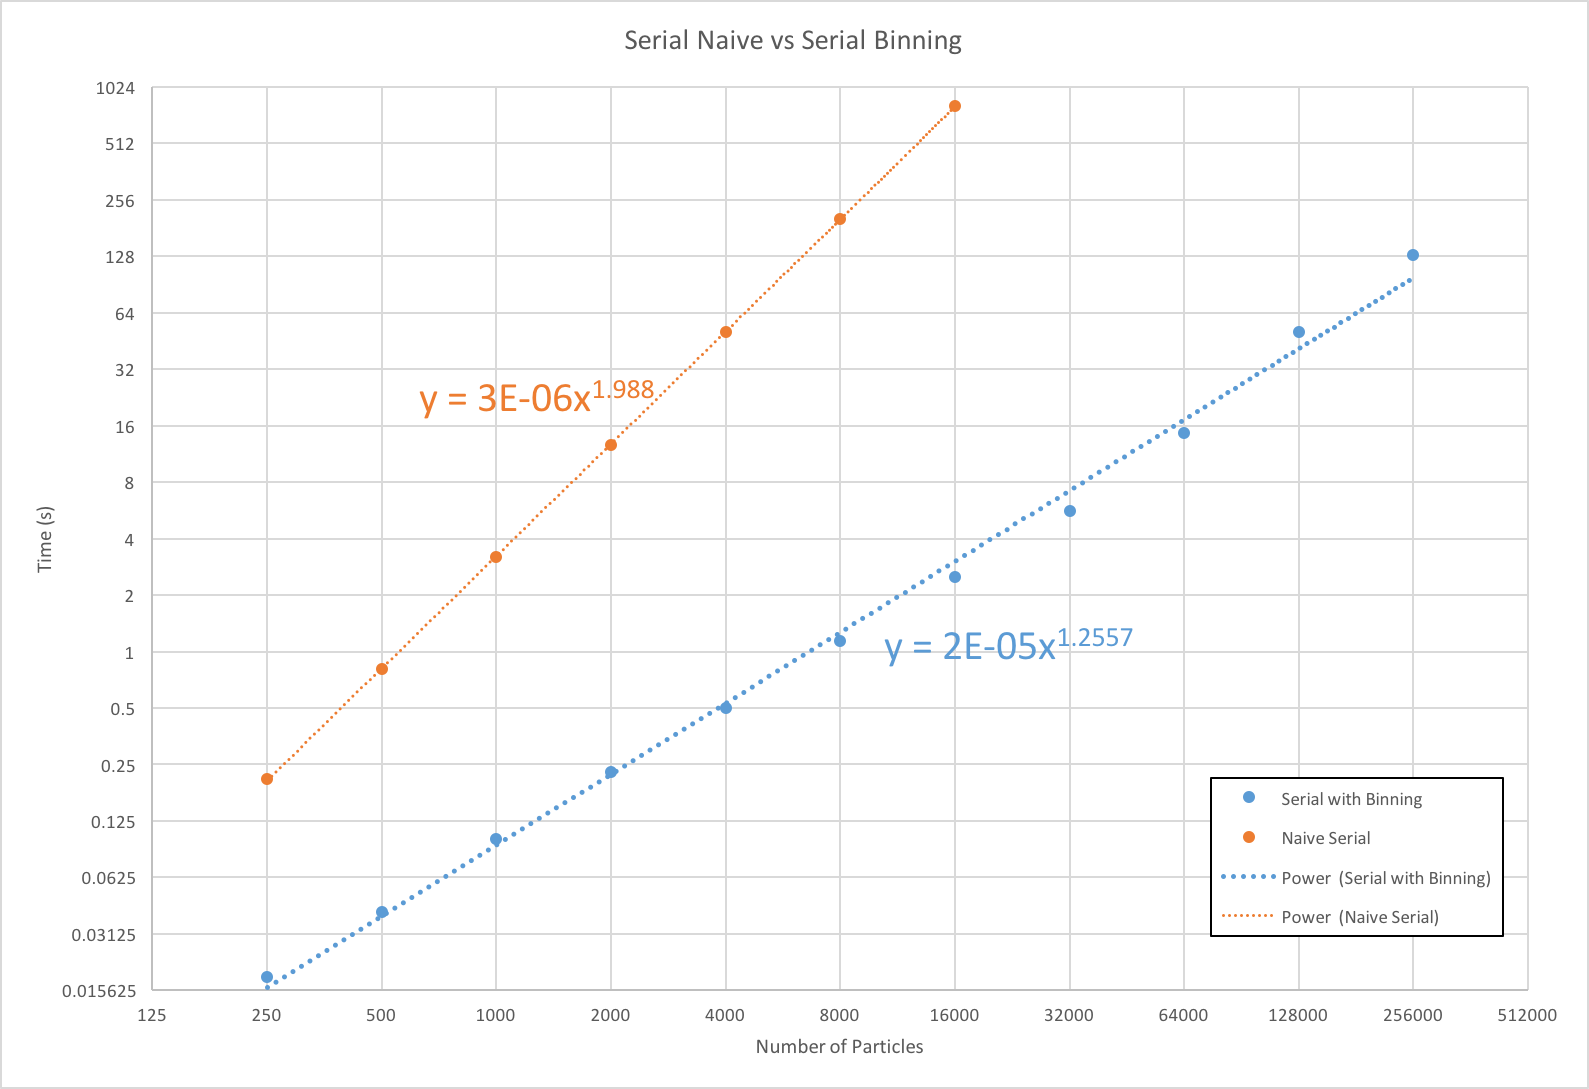
\includegraphics[width=\textwidth]{graphs/serial_binning_vs_naive.png}
  \caption{A plot in log-log scale that shows serial without binning runs on $O(n^2)$ time and serial with binning runs in $O(n)$ time.}
  \label{fig:serial-on}
\end{figure}

\section{OpenMP implementation}

\subsection{Synchronization}
%A description of the synchronization you used in the shared memory implementation.

We implement OpenMP for shared memory parallelization. Synchronization is used after each parallel region in order to prevent race conditions. First, we assign each particle to bins in parallel. Next, we assign each bin to a lock (using \texttt{omp\_lock\_t}). Bin sizes are about equal to the given cutoff size for particle interaction. Thus, the number of bins is generally higher than the number of particles. When we compute forces in each bin in parallel, there will be little contention in most bins because they are empty or relatively sparse. Lastly, we move each particle and clear each bin in parallel for the next timestep. 

\subsection{Results}

Figure \ref{fig:openmp-on} shows considerable speedup of our OpenMP implementation compared to serial binning using 12 threads. We compare based on 12 threads based on the strong scaling measurements in Figure \ref{fig:openmp-strong}. On average, the maximum speed is achieved with 12 threads for number of particles between 500 to 128,000. Four threads is faster below this range, and 24 threads is faster above this range. The simulation time for OpenMP is $O(n^{0.916})$, while the serial is $O(n^{1.256})$. 

Figure \ref{fig:openmp-strong} shows the strong scaling of our OpenMP implementation, or how the simulation time varies with the number of threads for a fixed total problem size. OpenMP scales as the number of particles exceeds 32,000. Figure \ref{fig:openmp-weak} shows the weak scaling of OpenMP, or how the computation time varies with the number of threads for a fixed problem size per thread. The slope of the linear scaling at 4,000 particles per thread is 0.088, whereas a slope of 0 would indicate that our code is flawless. There is more communication as the number of threads increases, which explains why the slope is not exactly 0.

\begin{figure}
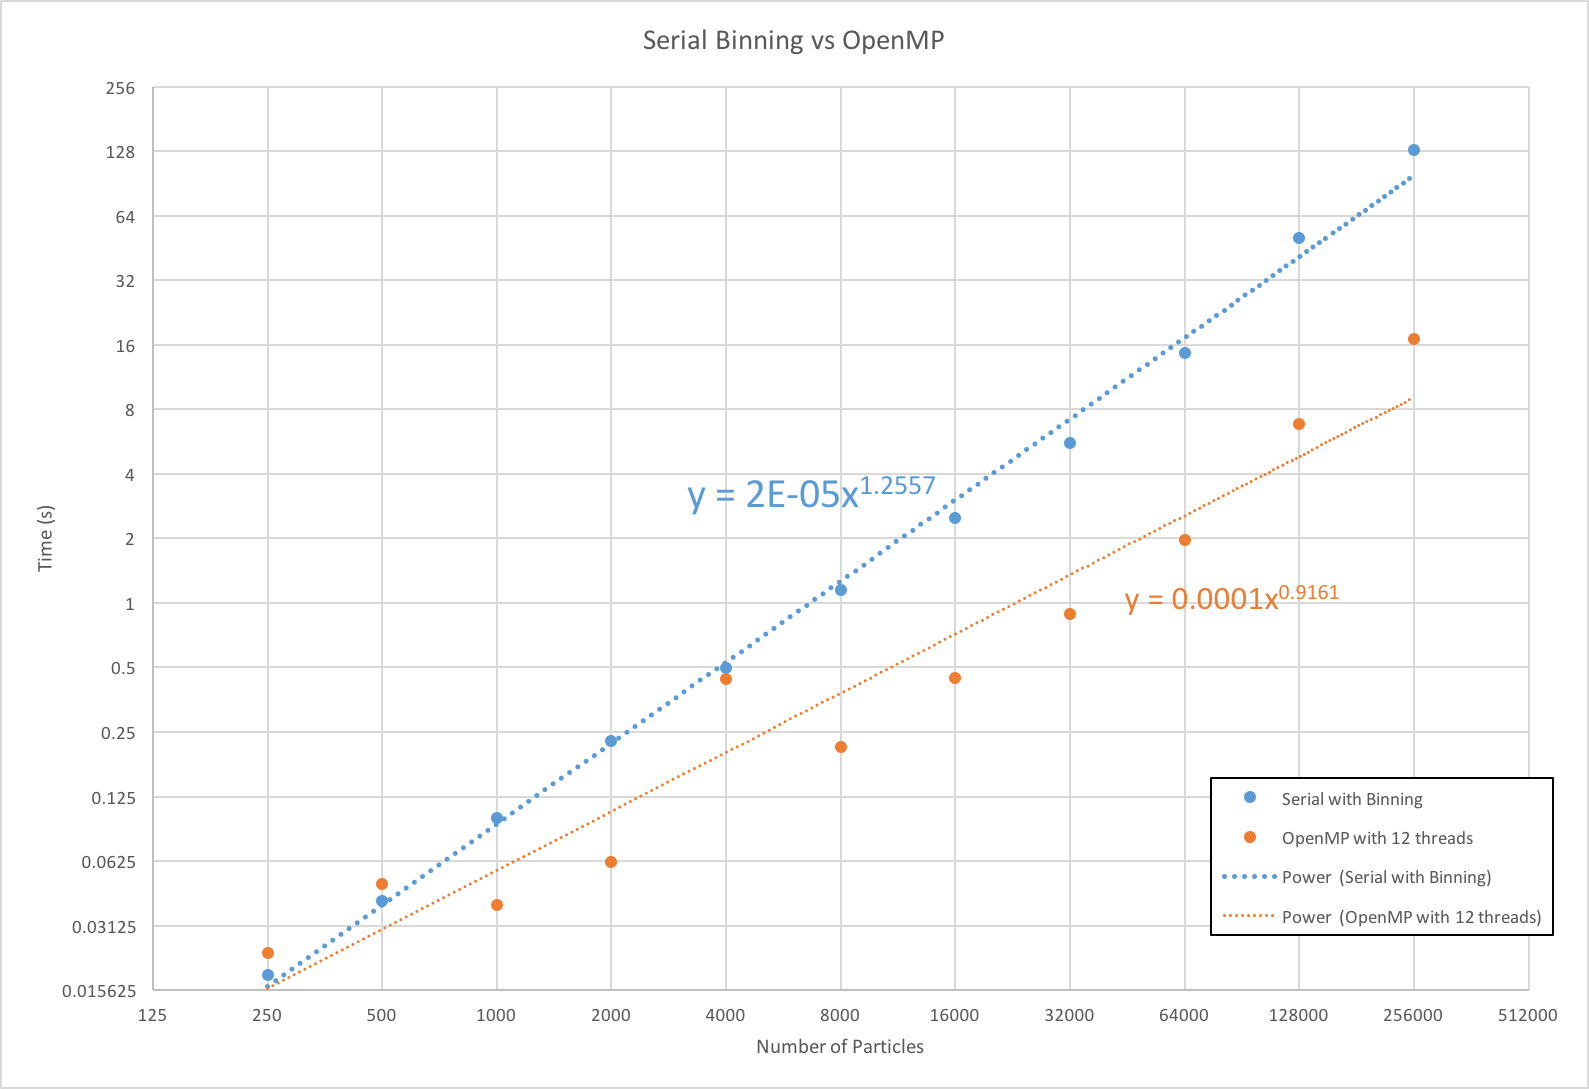
\includegraphics[width=\textwidth]{graphs/serial_binning_vs_openMP_12thr.png}
  \caption{$O(n)$ scaling of the OpenMP implementation with 12 threads compared to the serial implementation.}
  \label{fig:openmp-on}
\end{figure}

\begin{figure}
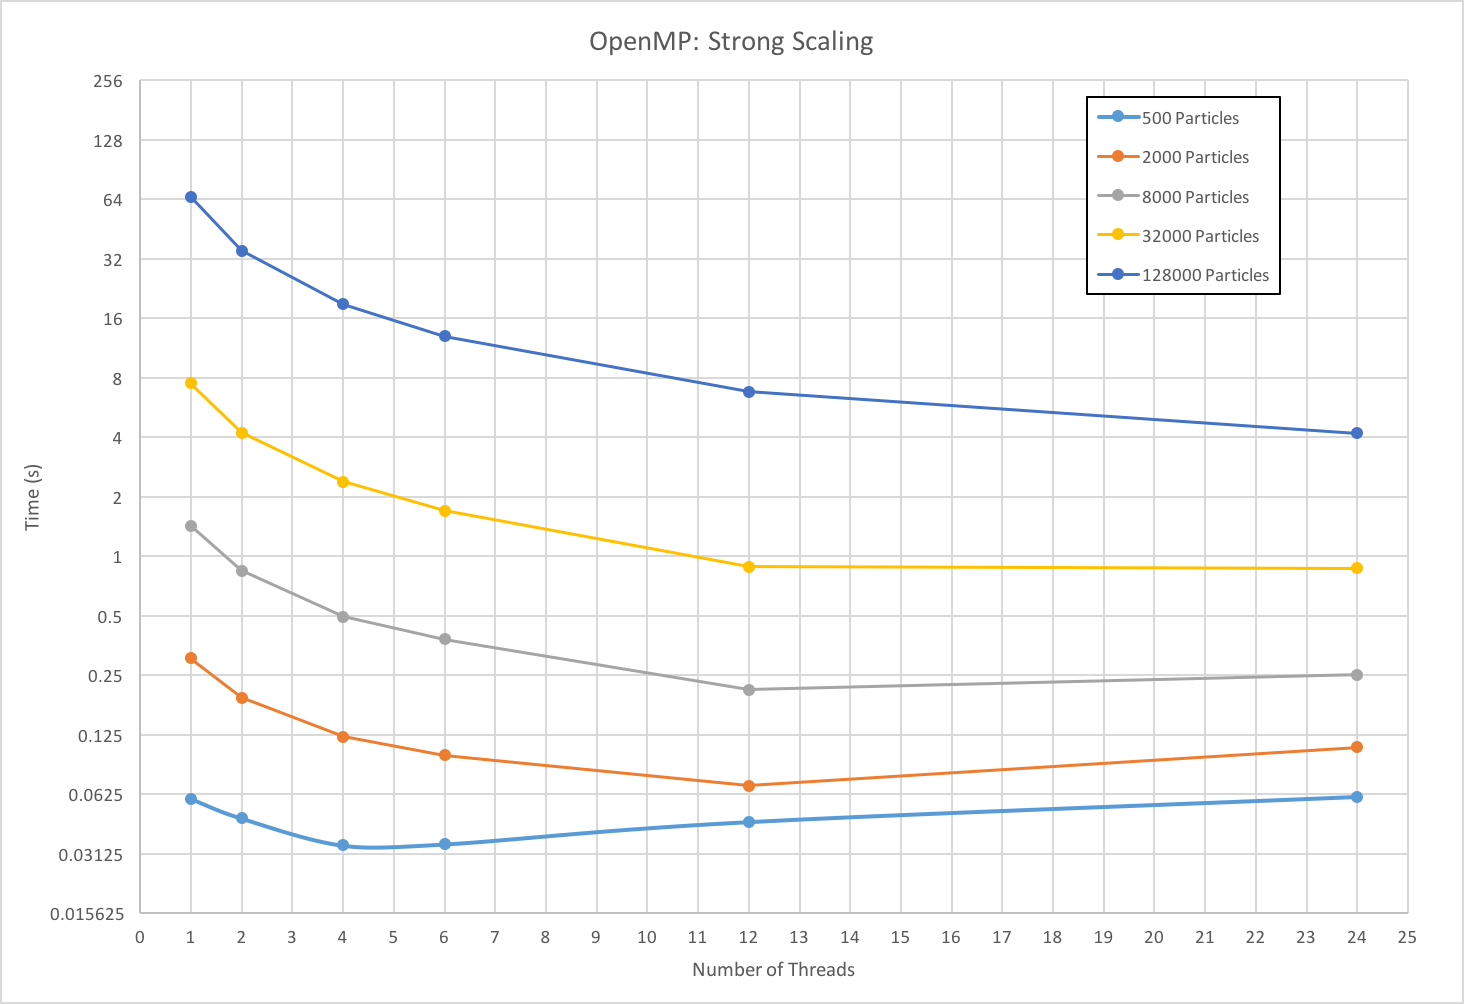
\includegraphics[width=\textwidth]{graphs/openmp_strong_scaling.png}
  \caption{Strong scaling of the OpenMP implementation.}
  \label{fig:openmp-strong}
\end{figure}

\begin{figure}
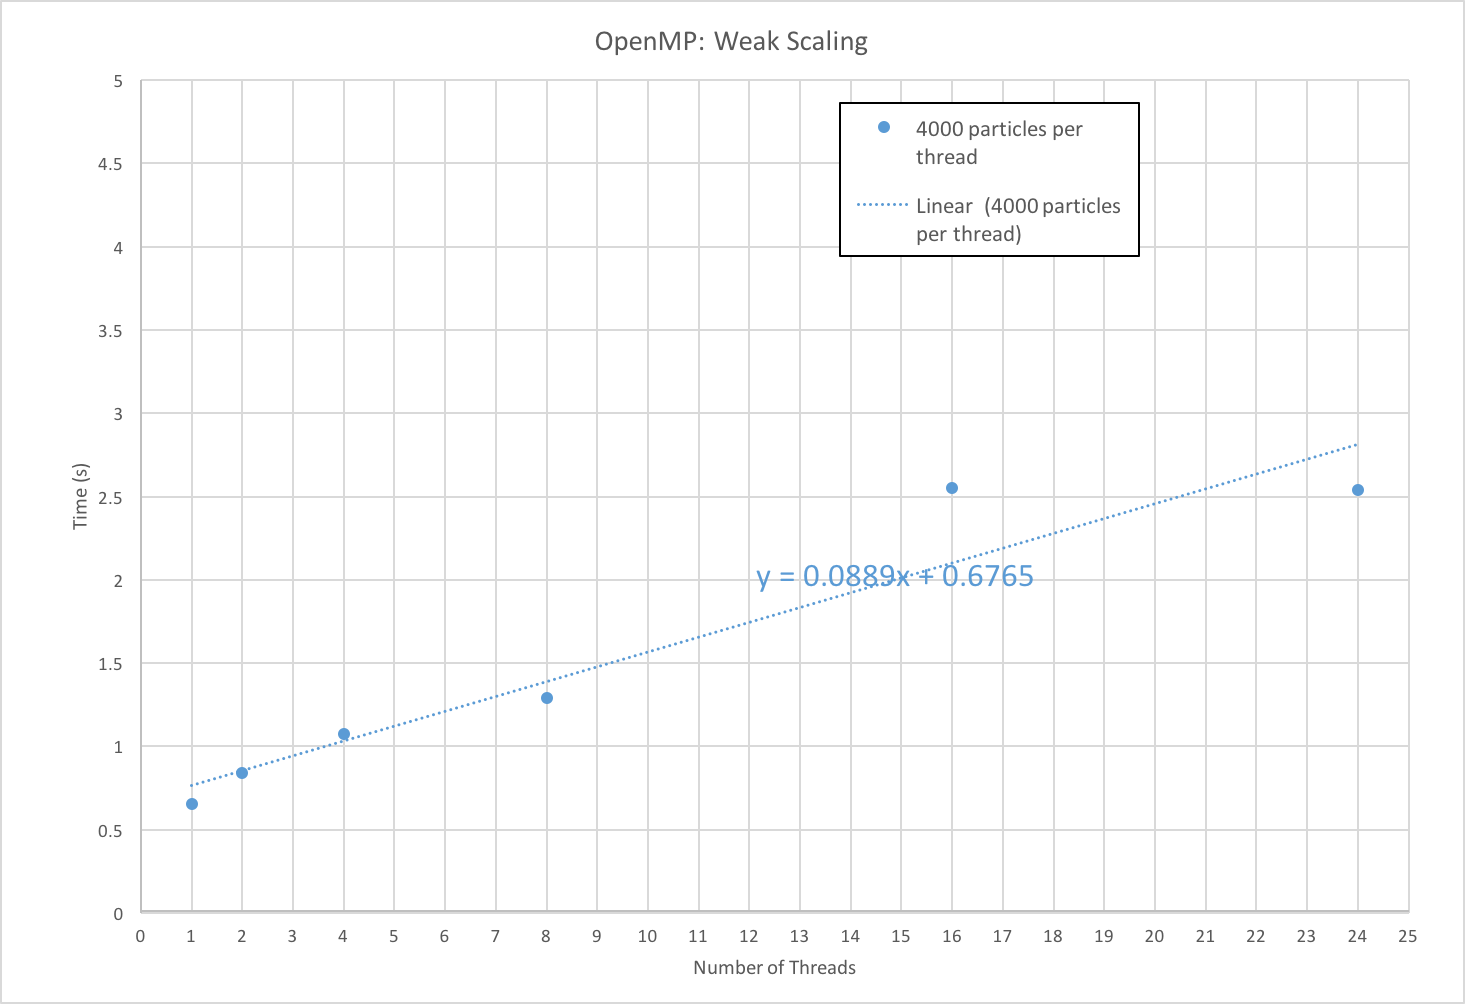
\includegraphics[width=\textwidth]{graphs/weak_scaling.png}
  \caption{Weak scaling of the OpenMP implementation.}
  \label{fig:openmp-weak}
\end{figure}

\section{MPI Implementation}

\subsection{Communication between nodes}
%A description of the communication you used in the distributed memory implementation.

\subsection{Results}

\begin{figure}
%  \includegraphics[width=\textwidth]{mpi-on.png}
  \caption{$O(n)$ scaling of the MPI implementation.}
  \label{fig:mpi-on}
\end{figure}

\begin{figure}
%  \includegraphics[width=\textwidth]{mpi-weak.png}
  \caption{Weak scaling of the MPI implementation.}
  \label{fig:mpi-weak}
\end{figure}

\begin{figure}
%  \includegraphics[width=\textwidth]{mpi-strong.png}
  \caption{Strong scaling of the MPI implementation.}
  \label{fig:mpi-strong}
\end{figure}

\subsection{Discussion}

%\begin{figure}
%  \includegraphics[width=\textwidth]{speedup.png}
%  \caption{Speedup plots that show how closely parallel codes approach the idealized $p$-times speedup.}
%  \label{fig:speedup}
%\end{figure}

%A description of the design choices that you tried and how did they affect the performance.

%A discussion on whether it is possible to do better

%A discussion on using pthreads, OpenMP and MPI.

\section{GPU Implementation} \label{GPU}

\subsection{Synchronization and GPU-specific optimizations}
%A description of any synchronization needed
%A description of any GPU-specific optimizations you tried

\subsection{Results}

%\begin{figure}
%  \includegraphics[width=\textwidth]{gpu-speedup.png}
%  \caption{A plot of the speedup of the GPU code versus the serial, openmp, mpi runs on the CPU of the node}
%  \label{fig:gpu-speedup}
%\end{figure}

\begin{figure}
 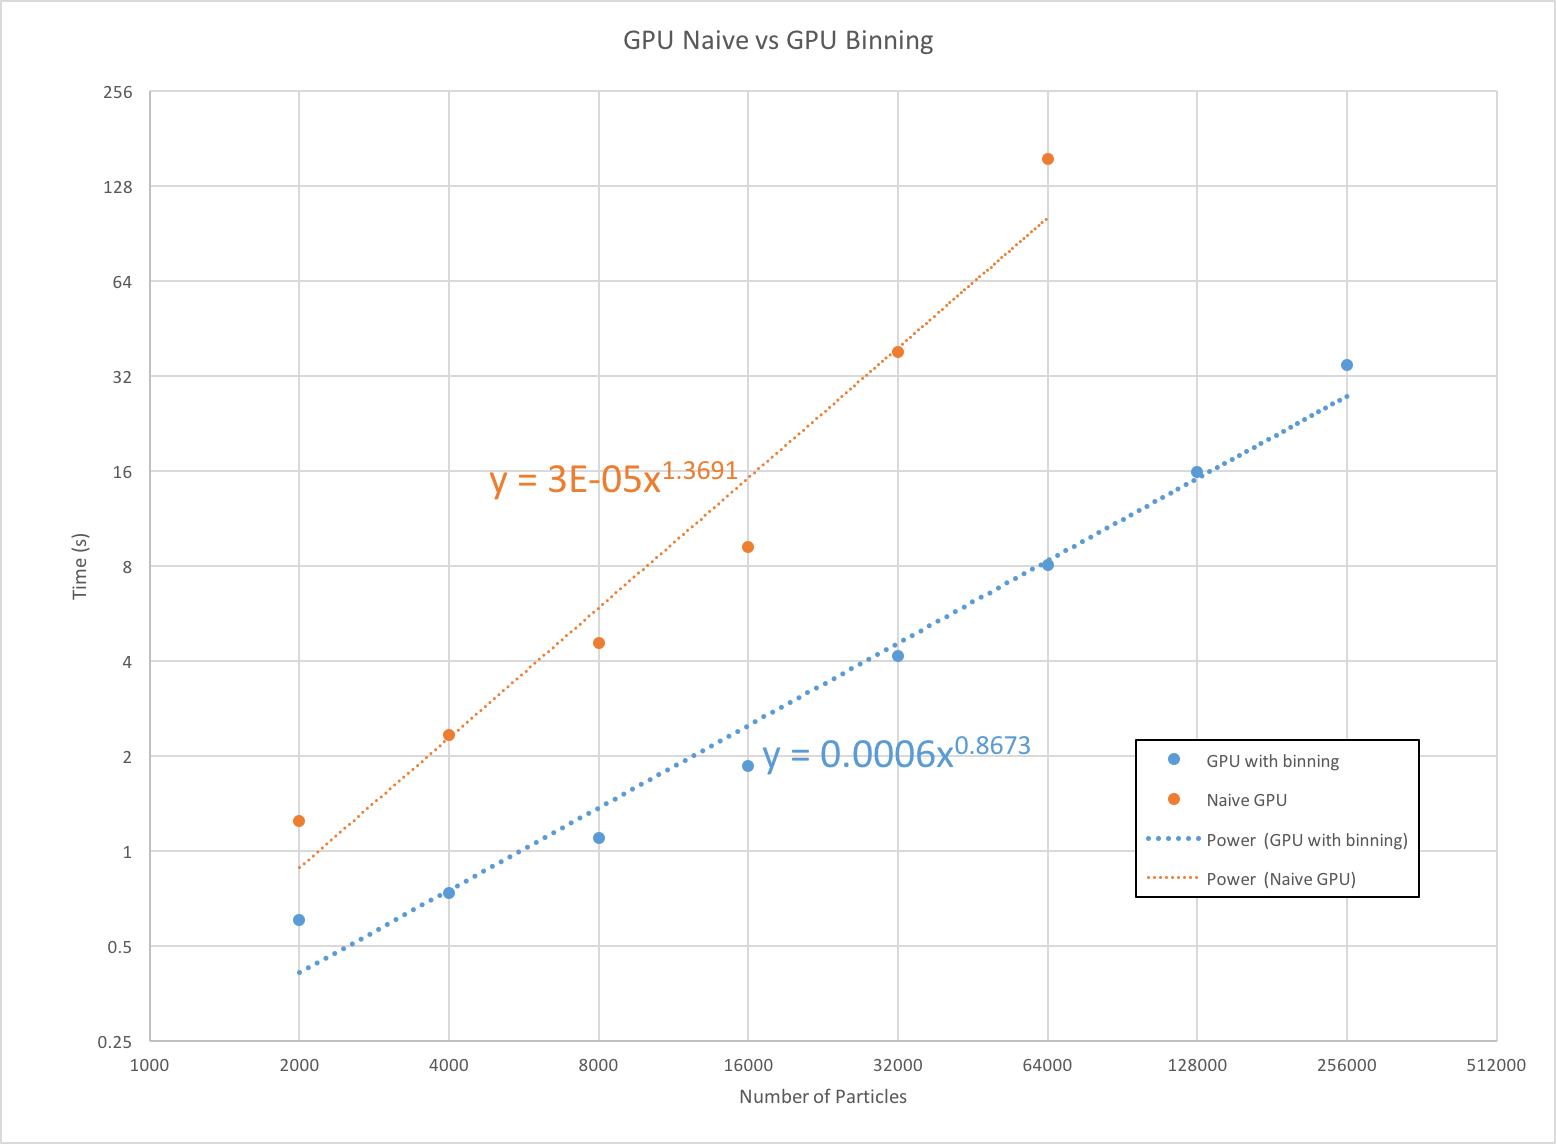
\includegraphics[width=\textwidth]{graphs/gpu_binning_vs_gpu_serial.png}
  \caption{Performance of GPU with binning versus the naive GPU code.}
  \label{fig:gpu-naive}
\end{figure}

\begin{figure}
 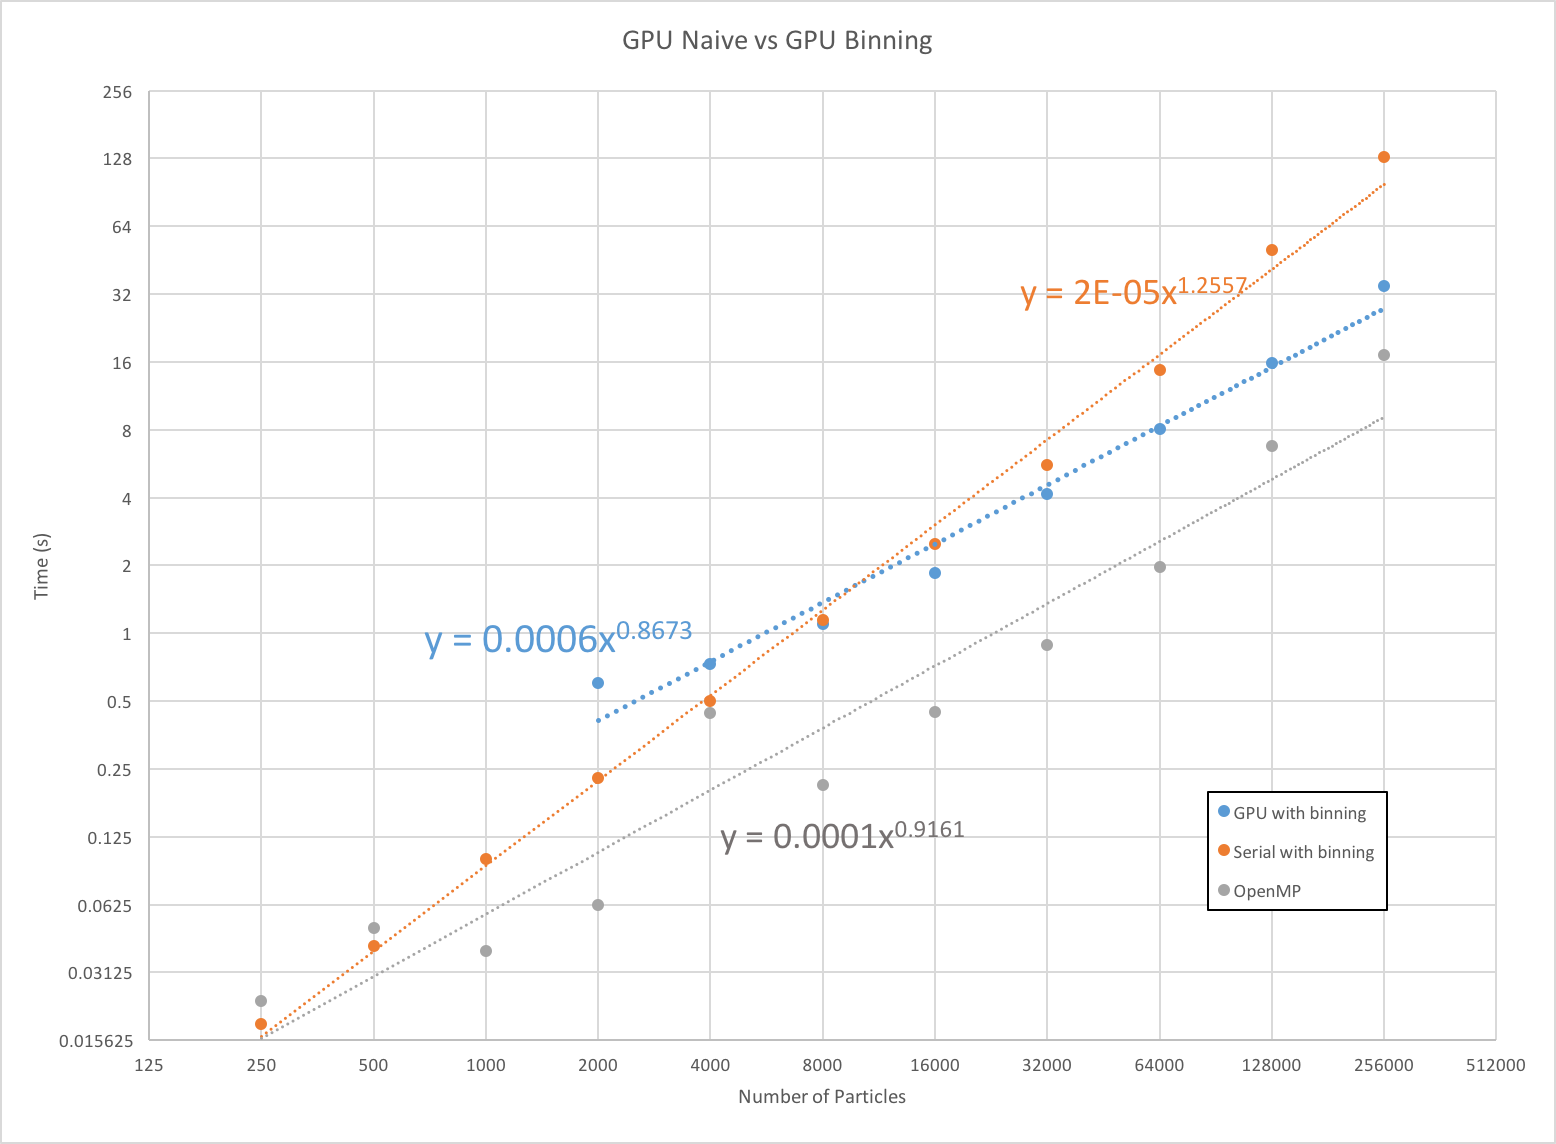
\includegraphics[width=\textwidth]{graphs/serial_openmp_gpu.png}
  \caption{Performance of GPU with binning versus serial with binning and parallelized OpenMP.}
  \label{fig:gpu-compare}
\end{figure}

\subsection{Discussion}
%A discussion on the strengths and weaknesses of CUDA and the current GPU architecture


%Appendix
%\pagebreak
%\begin{appendices}
%
%\end{appendices}

\end{document}
